\documentclass[10pt,landscape,a4paper]{article}
\usepackage[landscape,margin=0.5in]{geometry}
\usepackage{multicol}
\usepackage{amsmath,amssymb}
\usepackage{graphicx}
\usepackage{xcolor}
\usepackage{tikz}
\usepackage{booktabs}
\usepackage{enumitem}
\usepackage{fancyhdr}
\usepackage{titlesec}

% Compact formatting
\setlength{\parindent}{0pt}
\setlength{\parskip}{2pt}
\setlist[itemize]{leftmargin=*, noitemsep, topsep=0pt}
\setlist[enumerate]{leftmargin=*, noitemsep, topsep=0pt}

% Section formatting
\titleformat{\section}{\normalfont\large\bfseries\color{blue!70!black}}{\thesection}{1em}{}
\titleformat{\subsection}{\normalfont\normalsize\bfseries\color{blue!50!black}}{\thesubsection}{1em}{}
\titlespacing*{\section}{0pt}{6pt}{3pt}
\titlespacing*{\subsection}{0pt}{4pt}{2pt}

% Box for important formulas
\newcommand{\importantbox}[1]{%
  \fcolorbox{blue!50!black}{blue!5}{%
    \parbox{0.90\linewidth}{#1}%
  }%
}

% Red warning box
\newcommand{\warningbox}[1]{%
  \fcolorbox{red!70!black}{red!5}{%
    \parbox{0.90\linewidth}{#1}%
  }%
}

% Green insight box
\newcommand{\insightbox}[1]{%
  \fcolorbox{green!50!black}{green!5}{%
    \parbox{0.90\linewidth}{#1}%
  }%
}

% Purple definition box
\newcommand{\defbox}[1]{%
  \fcolorbox{purple!70!black}{purple!5}{%
    \parbox{0.90\linewidth}{#1}%
  }%
}

\pagestyle{fancy}
\fancyhf{}
\fancyhead[C]{\textbf{\raisebox{-8pt}{Moiety Conservation Laws -- Cheat Sheet 1.0}}}
\fancyfoot[C]{\thepage}
\renewcommand{\headrulewidth}{0.4pt}

\begin{document}

\begin{multicols}{3}

% =============================================================================
\section{Definitions}
% =============================================================================

\defbox{
\textbf{Moiety:} A subgroup of a larger molecule.

\textbf{Conserved Moiety:} A subgroup whose total amount remains constant during interconversion through a sequence of reactions.
}

\subsection{Examples of Conserved Moieties}
\begin{itemize}
\item Phosphate groups (ATP/ADP/AMP)
\item Proteins in phosphorylation cycles
\item NAD/NADH
\item Enzyme/enzyme-substrate (E/ES)
\item Coenzyme A
\end{itemize}

\subsection{Time Scale Separation}

Conservation is an \textbf{approximation}:
\begin{itemize}
\item Interconversions: \textbf{fast} (seconds--minutes)
\item Synthesis/degradation: \textbf{slow} (hours--days)
\end{itemize}

Over short time scales, total moiety $\approx$ constant.

% =============================================================================
\section{Simple Conserved Cycle}
% =============================================================================

\begin{center}
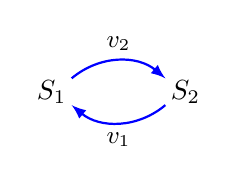
\begin{tikzpicture}[>=latex, scale=0.85]
\node at (0,0) {$S_1$};
\node at (2,0) {$S_2$};
\draw[->,thick,blue] (0.3,0.2) to[bend left=40] node[above,black] {\small $v_2$} (1.7,0.2);
\draw[->,thick,blue] (1.7,-0.2) to[bend left=40] node[below,black] {\small $v_1$} (0.3,-0.2);
\end{tikzpicture}
\end{center}

\subsection{System Equations}

\begin{align*}
\frac{ds_1}{dt} &= v_1 - v_2 \\[4pt]
\frac{ds_2}{dt} &= v_2 - v_1
\end{align*}

\importantbox{
\textbf{Key observation:}
\[ \frac{ds_1}{dt} = -\frac{ds_2}{dt} \]

Therefore: $s_1 + s_2 = T$ (constant)
}

\subsection{Reduced System}

Only need \textbf{one} ODE + \textbf{one} algebraic equation:

\importantbox{
\begin{align*}
s_2 &= T - s_1 \\[4pt]
\frac{ds_1}{dt} &= v_1 - v_2
\end{align*}
}

$T$ = total moiety (from initial conditions)

% =============================================================================
\section{Detecting Conservation Laws}
% =============================================================================

\subsection{Key Insight}

\importantbox{
\textbf{Row dependencies in $\mathbf{N}$} $\Leftrightarrow$ \textbf{Conservation laws}
}

For simple cycle:
\[
\mathbf{N} = \begin{bmatrix} 1 & -1 \\ -1 & 1 \end{bmatrix}
\]

Row 2 = $-1 \times$ Row 1 $\Rightarrow$ dependent rows!

\subsection{Counting}

\begin{center}
\small
\begin{tabular}{@{}ll@{}}
\toprule
\textbf{Quantity} & \textbf{Formula} \\
\midrule
Total species & $m$ \\
Rank of $\mathbf{N}$ & $r = \text{rank}(\mathbf{N})$ \\
Independent species & $r$ \\
Dependent species & $m - r$ \\
Conservation laws & $m - r$ \\
\bottomrule
\end{tabular}
\end{center}

\subsection{Three-Species Cycle Example}

\[
\mathbf{N} = \begin{bmatrix}
-1 & 0 & 1 \\
1 & -1 & 0 \\
0 & 1 & -1
\end{bmatrix}
\]

Sum of rows = 0, so:
\[ \frac{ds_1}{dt} + \frac{ds_2}{dt} + \frac{ds_3}{dt} = 0 \]

$\Rightarrow$ Conservation: $s_1 + s_2 + s_3 = T$

% =============================================================================
\section{Row Reduction Method}
% =============================================================================

\subsection{Algorithm}

\textbf{Step 1:} Form augmented matrix $[\mathbf{N} \mid \mathbf{I}]$

\textbf{Step 2:} Row reduce $\mathbf{N}$ to echelon form, applying same operations to $\mathbf{I}$

\textbf{Step 3:} Zero rows in reduced $\mathbf{N}$ $\Rightarrow$ corresponding rows in transformed $\mathbf{I}$ are conservation laws

\subsection{Mathematical Form}

After row reduction:
\[
\begin{bmatrix} \mathbf{M} \\ \mathbf{0} \end{bmatrix} \mathbf{v} =
\begin{bmatrix} \mathbf{X} \\ \mathbf{Y} \end{bmatrix} \frac{d\mathbf{S}}{dt}
\]

\importantbox{
The $\mathbf{Y}$ partition gives conservation laws:
\[ \mathbf{Y} \frac{d\mathbf{S}}{dt} = \mathbf{0} \]
}

\subsection{Worked Example}

Given linked cycles (E, ES, $S_1$, $S_2$):
\[
\mathbf{N} = \begin{bmatrix}
1 & 0 & -1 \\
0 & -1 & 1 \\
-1 & 1 & 0 \\
0 & 1 & -1
\end{bmatrix}
\]

After row reduction, extract bottom rows:
\[
\begin{bmatrix}
1 & 1 & 1 & 0 \\
0 & 1 & 0 & 1
\end{bmatrix}
\]

Conservation laws:
\begin{align*}
s_2 + es + s_1 &= T_1 \\
es + e &= T_2
\end{align*}

%\columnbreak

% =============================================================================
\section{Null Space Connection}
% =============================================================================

\importantbox{
The conservation matrix $\boldsymbol{\gamma}$ is the \textbf{null space} of $\mathbf{N}^T$:
\[ \mathbf{N}^T \boldsymbol{\gamma}^T = \mathbf{0} \]

Equivalently: $\boldsymbol{\gamma}$ is the \textbf{left null space} of $\mathbf{N}$:
\[ \boldsymbol{\gamma} \mathbf{N} = \mathbf{0} \]
}

\subsection{Verification Test}

To check if conservation laws are correct:
\[ \mathbf{N}^T \cdot (\text{conservation vectors}) = \mathbf{0} \]

\subsection{Software Commands}

\begin{center}
\small
\begin{tabular}{@{}ll@{}}
\toprule
\textbf{Tool} & \textbf{Command} \\
\midrule
MATLAB & \texttt{null(N', 'r')} \\
Scilab & \texttt{rref(kernel(N')')} \\
Python/SymPy & \texttt{Matrix(N).T.nullspace()} \\
Mathematica & \texttt{NullSpace[Transpose[N]]} \\
\bottomrule
\end{tabular}
\end{center}

% =============================================================================
\section{Matrix Partitioning}
% =============================================================================

\subsection{Stoichiometry Matrix Structure}

Reorder rows: independent ($\mathbf{S}_I$) on top, dependent ($\mathbf{S}_D$) on bottom:

\[
\mathbf{N} = \begin{bmatrix} \mathbf{N}_R \\ \mathbf{N}_0 \end{bmatrix}
\]

\begin{itemize}
\item $\mathbf{N}_R$: reduced matrix (full rank, $m_0 \times n$)
\item $\mathbf{N}_0$: dependent rows
\end{itemize}

\subsection{Link-Zero Matrix $\mathbf{L}_0$}

\importantbox{
$\mathbf{N}_0$ is a linear combination of $\mathbf{N}_R$:
\[ \mathbf{N}_0 = \mathbf{L}_0 \mathbf{N}_R \]
}

\vspace{5pt}
Dimensions: $\mathbf{L}_0$ is $(m - m_0) \times m_0$

\subsection{Link Matrix $\mathbf{L}$}

\[
\mathbf{L} = \begin{bmatrix} \mathbf{I} \\ \mathbf{L}_0 \end{bmatrix}
\]

\importantbox{
\textbf{Key relationship:}
\[ \mathbf{N} = \mathbf{L} \cdot \mathbf{N}_R \]
}

\vspace{5pt}
If no conservation: $\mathbf{L} = \mathbf{I}$

\subsection{Conservation Matrix}

\importantbox{
\[ \boldsymbol{\gamma} = \begin{bmatrix} -\mathbf{L}_0 & \mathbf{I} \end{bmatrix} \]

\vspace{-6pt}
Conservation law:
\vspace{-6pt}
\[ \boldsymbol{\gamma} \mathbf{S} = \mathbf{T} \]

\vspace{-6pt}
Or explicitly:
\vspace{-6pt}
\[ \begin{bmatrix} -\mathbf{L}_0 & \mathbf{I} \end{bmatrix} \begin{bmatrix} \mathbf{S}_I \\ \mathbf{S}_D \end{bmatrix} = \mathbf{T} \]
}

\subsection{Computing Dependent Species}

\importantbox{
\[ \mathbf{S}_D = \mathbf{L}_0 \mathbf{S}_I + \mathbf{T} \]
}

\vspace{4pt}
where $\mathbf{T} = \mathbf{S}_D(0) - \mathbf{L}_0 \mathbf{S}_I(0)$

% =============================================================================
\section{Reduced System}
% =============================================================================

\subsection{Full vs Reduced}

\textbf{Full system:} $m$ ODEs
\[ \frac{d\mathbf{S}}{dt} = \mathbf{N} \mathbf{v} \]

\textbf{Reduced system:} $m_0$ ODEs + $(m-m_0)$ algebraic
\begin{align*}
\frac{d\mathbf{S}_I}{dt} &= \mathbf{N}_R \mathbf{v} \\[4pt]
\mathbf{S}_D &= \mathbf{L}_0 \mathbf{S}_I + \mathbf{T}
\end{align*}

\subsection{Why Reduce?}

\begin{enumerate}
\item Fewer ODEs to integrate
\item Avoids numerical drift
\item Required for Jacobian inversion
\end{enumerate}

%\columnbreak

% =============================================================================
\section{Jacobian Implications}
% =============================================================================

\warningbox{
\textbf{Problem:} Conservation laws create \textbf{singular Jacobian}!

Row dependencies in $\mathbf{N}$ $\Rightarrow$ row dependencies in $\mathbf{J}$
}

\vspace{4pt}
For simple cycle with $v_1 = k_1 s_1$, $v_2 = k_2 s_2$:
\[
\mathbf{J} = \begin{bmatrix}
-k_1 & k_2 \\
k_1 & -k_2
\end{bmatrix}
\]

$\det(\mathbf{J}) = 0$ --- cannot invert!

\vspace{5pt}
\insightbox{
\textbf{Solution:} Work with the \textbf{reduced system} to get an invertible Jacobian.
}

% =============================================================================
\section{Numerical Methods}
% =============================================================================

\subsection{Method Comparison}

\begin{center}
\small
\begin{tabular}{@{}lcc@{}}
\toprule
\textbf{Method} & \textbf{Stability} & \textbf{Speed} \\
\midrule
Row reduction & Poor & Fast \\
SVD & Excellent & Slow \\
QR factorization & Excellent & Medium \\
\bottomrule
\end{tabular}
\end{center}

\subsection{SVD Method}

Factor $\mathbf{N}^T = \mathbf{U} \mathbf{S} \mathbf{V}^T$

Null space = bottom rows of $\mathbf{V}^T$ (where $\sigma_i = 0$)

Apply \texttt{rref()} for rational basis.

\subsection{QR Method}

Factor $\mathbf{N}^T \mathbf{P} = \mathbf{Q} \mathbf{R}$

Extract $\mathbf{L}_0$ from reduced $\mathbf{R}$:
\[ \mathbf{L}_0 = \mathbf{R}_{12}^T \]

after row reducing top portion.

\subsection{Best Practice}

\insightbox{
\textbf{Row ordering tip:} Place \textbf{shared species} (complexes) at \textbf{bottom} of $\mathbf{N}$ to get positive conservation law coefficients.
}

% =============================================================================
\section{Multicompartment Systems}
% =============================================================================

\warningbox{
\textbf{Conservation is of MASS, not concentration!}

For cross-compartment conservation:
\[ \sum_i V_i s_i = T \]

where $V_i$ = volume of compartment $i$
}

% =============================================================================
\section{Summary of Key Equations}
% =============================================================================

\begin{center}
\small
\begin{tabular}{@{}ll@{}}
\toprule
\textbf{Relation} & \textbf{Equation} \\
\midrule
Full system & $\mathbf{N} = \mathbf{L} \mathbf{N}_R$ \\[4pt]
Link-zero & $\mathbf{N}_0 = \mathbf{L}_0 \mathbf{N}_R$ \\[4pt]
Conservation matrix & $\boldsymbol{\gamma} = [-\mathbf{L}_0 \mid \mathbf{I}]$ \\[4pt]
Null space & $\mathbf{N}^T \boldsymbol{\gamma}^T = \mathbf{0}$ \\[4pt]
Conservation law & $\boldsymbol{\gamma} \mathbf{S} = \mathbf{T}$ \\[4pt]
Dependent species & $\mathbf{S}_D = \mathbf{L}_0 \mathbf{S}_I + \mathbf{T}$ \\
\bottomrule
\end{tabular}
\end{center}

% =============================================================================
\section{Quick Reference: Tellurium}
% =============================================================================

{\small
\begin{verbatim}
import tellurium as te
r = te.loada('''
  S1 -> S2; k1*S1
  S2 -> S1; k2*S2
  S1 = 10; k1 = 0.1; k2 = 0.2
''')
r.conservedMoietyAnalysis = True
print(r.getConservationMatrix())
print(r.getLinkMatrix())
\end{verbatim}
}

\vfill
\hrule
\vspace{3pt}
\footnotesize
\textit{Based on: H.M. Sauro, ``Systems Biology: Introduction to Pathway Modeling'', Created: \today}

\end{multicols}
\end{document}
